\documentclass[12pt]{article}
% controlling the geometry of the page:
\usepackage[margin=1in, paperwidth=8.5in, paperheight=11in]{geometry} 
\usepackage{amsmath, amssymb} % useful math symbols and environments

\usepackage{multicol} % multiple columns side-by-side

\usepackage{amsthm} % Theorem-like environments
\theoremstyle{definition} % Without this line, theorem statements (and therefore problem statements etc.) show up in italic text.
\newtheorem{conjecture}{Conjecture}
\newtheorem{problem}{Problem}

% pretty colors!
\usepackage[dvipsnames]{xcolor}
\colorlet{darkgrey}{black!70}
\colorlet{darkgreen}{green!50!black}

\usepackage{tikz} % for drawing diagrams
\usetikzlibrary{arrows,automata,positioning} 
\usetikzlibrary{decorations.markings}
\usetikzlibrary{decorations.pathreplacing}
\usetikzlibrary{patterns}
\usetikzlibrary{shapes.geometric}

%%---------------------------------------------------------------------------
%% included from visualalgebra.sty (see the beamer folder)
%% TEXT COLORS
%%
\definecolor{xRed}{rgb}{.9,0,0}       
\definecolor{xBlue}{rgb}{0,0,.9}      
\definecolor{xGreen}{HTML}{009000}   %% "Islamic green"
\definecolor{xPurple}{HTML}{D14FFF}  
\definecolor{xOrange}{HTML}{F56600}  %% "Clemson orange"

\newcommand{\Alert}[1]{\textcolor{xRed}{#1}}
\newcommand{\Balert}[1]{\textcolor{xBlue}{#1}}
\newcommand{\Galert}[1]{\textcolor{xGreen}{#1}}
\newcommand{\Palert}[1]{\textcolor{xPurple}{#1}}
\newcommand{\Oalert}[1]{\textcolor{xOrange}{#1}}
\newcommand{\Walert}[1]{\textcolor{white}{#1}}

%% vertices in cayley graphs
\tikzset{v/.style={circle, draw, fill=lightgray,inner sep=0pt, 
  minimum size=6mm}}

%% Edge colors
%%
\definecolor{eRed}{rgb}{1,0,0}      % Cayley diagram edges
\definecolor{eBlue}{rgb}{0,0,1}     % Cayley diagram edges
\definecolor{eGreen}{HTML}{7EC636}  % Goodnotes green (a little darker)
\definecolor{eGreen}{HTML}{3CAC13}  % I like this a litte better
\definecolor{ePurple}{HTML}{D287FF} % Close to goodnotes 
\colorlet{eOrange}{orange}

%% Edge styles 
%%
\tikzset{r/.style={draw, very thick, eRed, -stealth}}  % Red -->
\tikzset{rr/.style={draw, very thick, eRed}}           % Red ---
\tikzset{b/.style={draw, very thick, eBlue, -stealth}} % Blue -->
\tikzset{bb/.style={draw, very thick, eBlue}}          % Blue ---
\tikzset{g/.style={draw, very thick, eGreen, -stealth}} % Green -->
\tikzset{gg/.style={draw, very thick, eGreen}}          % Green ---
%%---------------------------------------------------------------------------

\usepackage{graphicx} % for inserting figures with \includegraphics
\usepackage{setspace} % for controlling space between lines, paragraphs, etc.

\usepackage{fancyhdr} % for controlling headers and footers
\usepackage{newtx} % changes the default font family
\usepackage[shortlabels]{enumitem} % controllable labels for ordered and unordered lists

\usepackage{hyperref} % controls hyperlinks, both internal and external
\hypersetup{
    colorlinks=true,
    urlcolor=blue,
}

\setlength{\headheight}{14.5pt}
\newcommand{\Q}{\mathbb{Q}}
\newcommand{\R}{\mathbb{R}}
\newcommand{\Z}{\mathbb{Z}}
\newcommand\inv{^{-1}} % I am very tired of typing ^{-1}
\def\<{\langle}
\def\>{\rangle}
\DeclareMathOperator\Rect{\mathbf{Rect}}
\DeclareMathOperator\Tri{\mathbf{Tri}}
\DeclareMathOperator\Sq{\mathbf{Sq}}
\DeclareMathOperator\Light{\mathbf{Light}}
\DeclareMathOperator{\lcm}{lcm}

\newenvironment{red}{\color{red}}{\ignorespacesafterend}
\newenvironment{xBlue}{\color{xBlue}}{\ignorespacesafterend}

% I don't like how LaTeX renders section headings by default
\renewcommand{\section}[1]{\begin{center} \textbf{#1} \\\end{center}}
%
\setlength{\parindent}{0in}
%\oddsidemargin=-.25in
\allowdisplaybreaks
\pagestyle{fancy}
\renewcommand{\headrulewidth}{0pt}
\lhead{MATH 312}
\rhead{Spring 2025}
%\lfoot{\copyright\ CLEAR Calculus 2010}
\cfoot{}
\renewcommand{\thefootnote}{*} 
\hyphenpenalty=10000 % LaTeX by default really likes hyphenating things

% all the stuff above this line is called the preamble...
%##################################################################
\begin{document} % this is always the first line of what's actually produced
\section{Homework \#3 -- \Alert{Key}} % notice that if you want the character # to appear, you have to "escape" it with a backslash

HW due Sunday 2/9 by pdf upload to Canvas; .tex source on the \href{https://github.com/rhinopotamus/math312}{MATH 312 github repo}.

\subsection*{Stuff about permutation groups and $S_n$}

\begin{problem} (Omitted from key bc any reasonable explanation is correct.)
\end{problem}

\begin{problem}
    Suppose that $g, h \in G$. We mentioned in class that the \textit{conjugate} of $h$ by $g$ is the element $ghg\inv$. The \textit{conjugacy class} of $h$ is the set of all the possible conjugates of $h$: $\{ghg\inv \mid g\in G\}.$
    \begin{itemize}
        \item Find the conjugacy classes of all six elements of $S_3$. (If you use the permutation calculator, make sure you're multiplying left-to-right!) 
        \begin{red}
            \begin{itemize}
                \item Identity: $\{e\}$
                \item Transpositions: $\{(1\;2), (1\;3), (2\;3)\}$
                \item 3-cycles: $\{(1\;2\;3), (1\;3\;2)\}$
            \end{itemize}
        \end{red}
        \item If you are having fun, find the conjugacy classes of all 24 elements of $S_4$.
        \begin{red}
            \begin{itemize}
                \item Identity: $\{e\}$
                \item Transpositions: $\{(1\;2), (1\;3), (1\;4), (2\;3), (2\;4), (3\;4)\}$
                \item Double transpositions: $\{(1\;2)(3\;4), (1\;3)(2\;4), (1\;4)(2\;3)\}$
                \item 3-cycles: $\{(1\;2\;3), (1\;3\;2), (1\;2\;4), (1\;4\;2),
                (1\;3\;4),(1\;4\;3),(2\;3\;4),(2\;4\;3)\}$
                \item 4-cycles: $\{(1\;2\;3\;4), (1\;2\;4\;3), (1\;3\;2\;4), (1\;3\;4\;2), (1\;4\;2\;3), (1\;4\;3\;2)\}$
            \end{itemize}
        \end{red}
    \end{itemize}
\end{problem}

\begin{problem}
    Suppose $\sigma \in S_n$, and that $|\sigma| = k$. 

    \begin{red}
        Please note that I am writing out the details of this proof very carefully, so that it is clear at each step what is my data and what is my claim. As is usual, most of the warrants are ``implicit;'' see if you can fill in the warrants that connect the data to the claims.
    \end{red}
    \begin{itemize}
        \item Explain why $\sigma^k$ is an even permutation.

        \begin{red}
            Since $|\sigma| = k$, $\sigma^k = e$. The identity permutation $e$ is an even permutation, as it takes 0 transpositions to write. Therefore, $\sigma^k$ is an even permutation.
        \end{red}
        \item Suppose that $\sigma$ is an odd permutation. Is $k$ even or odd? How do you know?

        \begin{red}
            Let $t$ be the number of transpositions it takes to write $\sigma$. Since $\sigma$ is an odd permutation, we know that $t$ is an odd number.

            Now consider $\sigma^k = \underbrace{\sigma \cdot \sigma \cdot \ldots \cdot \sigma}_{k \text{ times}}$. How many total transpositions is that? Since each copy of $\sigma$ represents $t$ transpositions, $\sigma^k$ represents $t\cdot k$ total transpositions. 

            But $\sigma^k = e$ is an even transposition, so $t\cdot k$ must be an even number. Therefore, since $t$ is odd, $k$ must be even.
        \end{red}
        \item Conclude that a cycle of odd length is an even permutation. Feel moderate annoyance.

        \begin{red}
            The order of a cycle is the same as its length. For instance, the order of a transposition like $(1\;3)$ is 2; the order of a 3-cycle like $(1\;2\;3)$ is 3. 

            Suppose $\sigma$ is a cycle of odd length. Therefore its order must also be odd. So, if $|\sigma| = k$, then $k$ is an odd number.

            Again, let $t$ be the number of transpositions it takes to write $\sigma$. Again, $\sigma^k$ requires $t\cdot k$ transpositions to write. Since $\sigma^k = e$, which is an even permutation, we know that $t\cdot k$ must be an even number.

            Now, since $t\cdot k$ is an even number but $k$ is an odd number, we conclude that $t$ is an even number. Therefore $\sigma$ is an even permutation, by the definition of even permutations.
        \end{red}
    \end{itemize}
\end{problem}

\begin{problem}
    Play a bit more with Cayley's theorem:
    \begin{itemize}
        \item Extract from the Cayley diagram of $C_4\times C_2 = \< \Alert{r}, \Balert{b} \>$ the two permutations that describe its arrows, and therefore describe $C_4 \times C_2$ as a subgroup of a symmetric group.

        \begin{red}
            A key step in this process is to relabel the nodes with the numbers 1-8 (in this case; if the group had order 12 then it'd be the numbers 1-12, etc.). It doesn't really matter how you choose to number the nodes, but you do have to number them. To make my point, I've chosen labels for both $C_4 \times C_2$ and $Q_8$ that I don't think anybody else would have used.
        \end{red}

        {\color{red} With the number labels I've assigned in the diagram below,} 
        \[C_4 \times C_2 \cong \<\Alert{(1\;3\;5\;7)(2\;4\;6\;8)}, \Balert{(1\;2)(3\;4)(5\;6)(7\;8)}\>.\]
        
        \item Do the same for $Q_8 = \< \Alert{i}, \Balert{j}, \Galert{-1} \>$.

        {\color{red} With the number labels I've assigned in the diagram below,} 
        \[Q_8 \cong \<\Alert{(1\;2\;5\;6)(3\;4\;7\;8)}, \Balert{(1\;4\;5\;8)(2\;3\;6\;7)}, \Galert{(1\;5)(2\;6)(3\;7)(4\;8)}\>.\]

        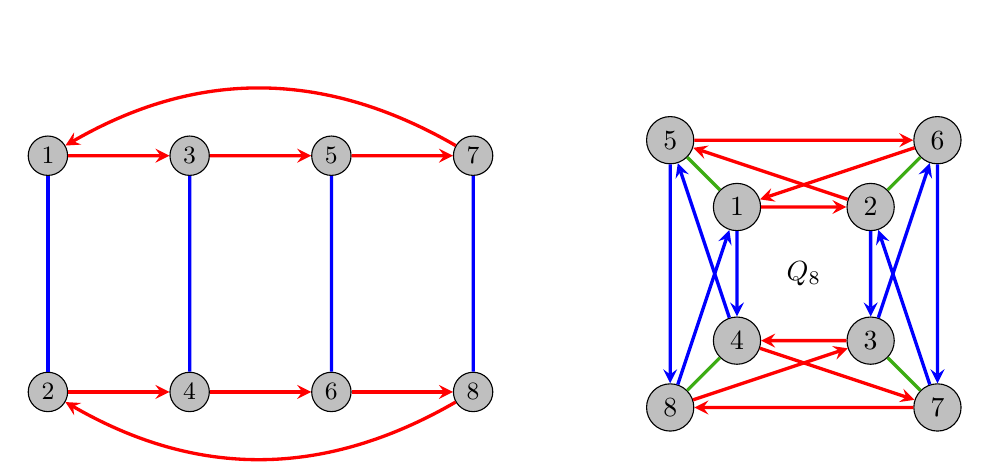
\begin{tikzpicture}[scale = 1.2]
            \begin{scope}[shift = {(-4, 0)}]
                \tikzstyle{v} = [circle, draw, fill=lightgray,inner sep=0pt, 
                    minimum size=5mm]  
                \tikzstyle{every node}=[font=\small]
                %%
                \node (10) at (0,2.5) [v] {$1$};
                \node (11) at (1.5,2.5) [v] {$3$};
                \node (12) at (3,2.5) [v] {$5$};
                \node (13) at (4.5,2.5) [v] {$7$};
                \node (00) at (0,0) [v] {$2$};
                \node (01) at (1.5,0) [v] {$4$};
                \node (02) at (3,0) [v] {$6$};
                \node (03) at (4.5,0) [v] {$8$};
                \draw [r] (00) to (01); 
                \draw [r] (01) to (02);
                \draw [r] (02) to (03);
                \draw [r] (03) to [bend left] (00);
                \draw [r] (10) to (11); 
                \draw [r] (11) to (12);
                \draw [r] (12) to (13);
                \draw [r] (13) to [bend right] (10);
                \draw [bb] (00) to (10);
                \draw [bb] (01) to (11);
                \draw [bb] (02) to (12);
                \draw [bb] (03) to (13);
            \end{scope}
            \begin{scope}[shift = {(4, 1.25)}]
                \node (1) at (135:1) [v] {$1$};
                \node (i) at (45:1) [v] {$2$};
                \node (k) at (-45:1) [v] {$3$};
                \node (j) at (-135:1) [v] {$4$};
                \node (-1) at (135:2) [v] {$5$};
                \node (-i) at (45:2) [v] {$6$};
                \node (-k) at (-45:2) [v] {$7$};
                \node (-j) at (-135:2) [v] {$8$};
                \node at (0,0) {\normalsize $Q_8$};
                %%
                \path[r] (1) to (i);
                \path[r] (i) to (-1);
                \path[r] (-1) to (-i);
                \path[r] (-i) to (1);
                %%
                \path[r] (k) to (j);
                \path[r] (j) to (-k);
                \path[r] (-k) to (-j);
                \path[r] (-j) to (k);
                %%
                \path[b] (i) to (k);
                \path[b] (k) to (-i);
                \path[b] (-i) to (-k);
                \path[b] (-k) to (i);
                %%
                \path[b] (1) to (j);
                \path[b] (j) to (-1);
                \path[b] (-1) to (-j);
                \path[b] (-j) to (1);
                %%
                \path[gg] (1) to (-1);
                \path[gg] (j) to (-j);
                \path[gg] (i) to (-i);
                \path[gg] (k) to (-k);
            \end{scope}
          \end{tikzpicture}
    \end{itemize}
    
\end{problem}

\subsection*{Stuff about direct products}

\begin{problem}
    I want to make the relationship between the inflate-the-Cayley-diagram description and the ordered-pairs description of a direct product a bit more evident. Say that $\Alert{C_4} = \<\Alert{r} \mid \Alert{r}^4 = 1\>$ and $\Balert{C_3} = \< \Balert{b} \mid \Balert{b}^3 = 1\>$. 
    \begin{itemize}
        \item Write out all 12 elements of $\Alert{C_4}\times \Balert{C_3}$ as ordered pairs. (They will all look like $(\Alert{r}^k, \Balert{b}^j)$.)
        \[
        \begin{array}{cccc}
            (\Alert{1}  , \Balert{1}) & 
            (\Alert{r}  , \Balert{1}) &
            (\Alert{r^2}, \Balert{1}) &
            (\Alert{r^3}, \Balert{1}) \\
            (\Alert{1}  , \Balert{b}) & 
            (\Alert{r}  , \Balert{b}) &
            (\Alert{r^2}, \Balert{b}) &
            (\Alert{r^3}, \Balert{b}) \\
            (\Alert{1}  , \Balert{b^2}) & 
            (\Alert{r}  , \Balert{b^2}) &
            (\Alert{r^2}, \Balert{b^2}) &
            (\Alert{r^3}, \Balert{b^2})
        \end{array}
        \]
        \item Use the inflation procedure to draw the Cayley diagram of $\Alert{C_4}\times \Balert{C_3}$.
        \item Label each node in your Cayley diagram with the corresponding ordered pair.

        \begin{red}
            I am emphasizing that it is 100\% fine to draw your diagram by hand. It took me, and I timed it, 14 minutes to draw these two diagrams, and that includes going upstairs to get new markers. I promise it would have taken me way longer than that to do this in tikz. 
        \end{red}

        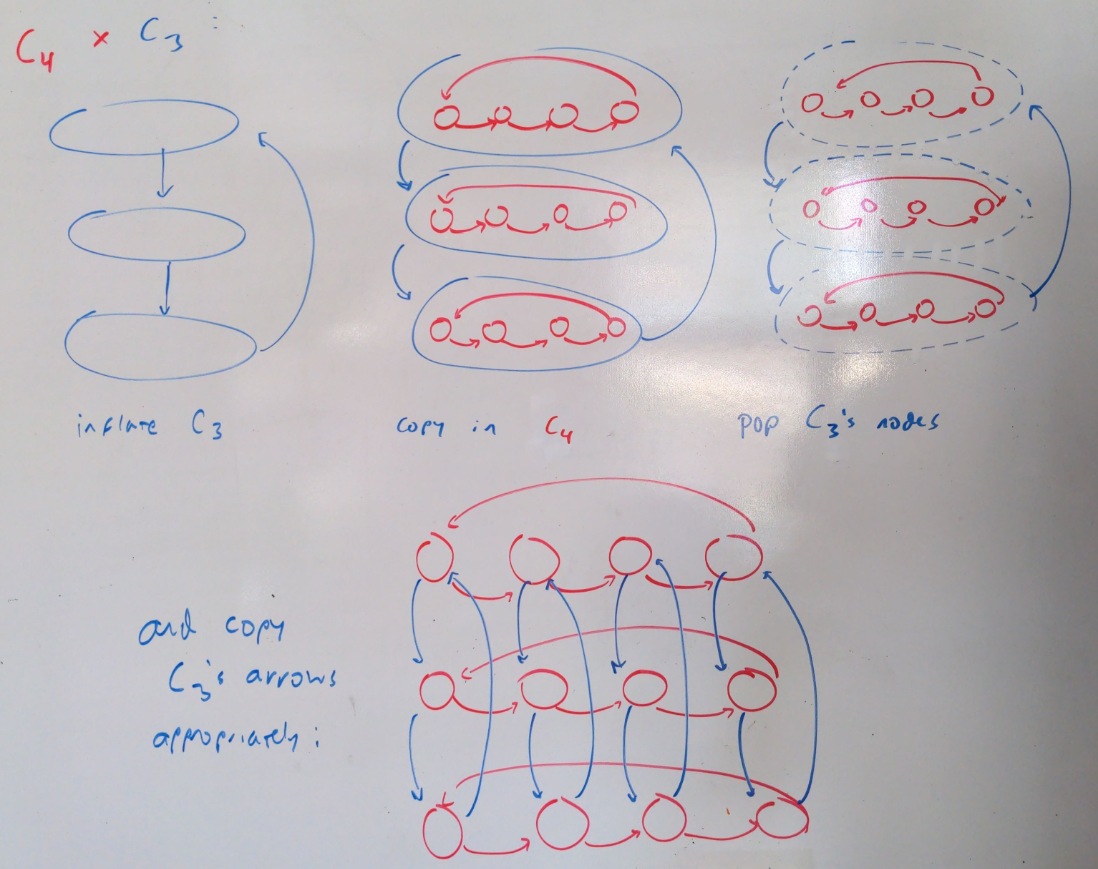
\includegraphics[width=0.5\textwidth]{../images/c4c3-inflation.png}
        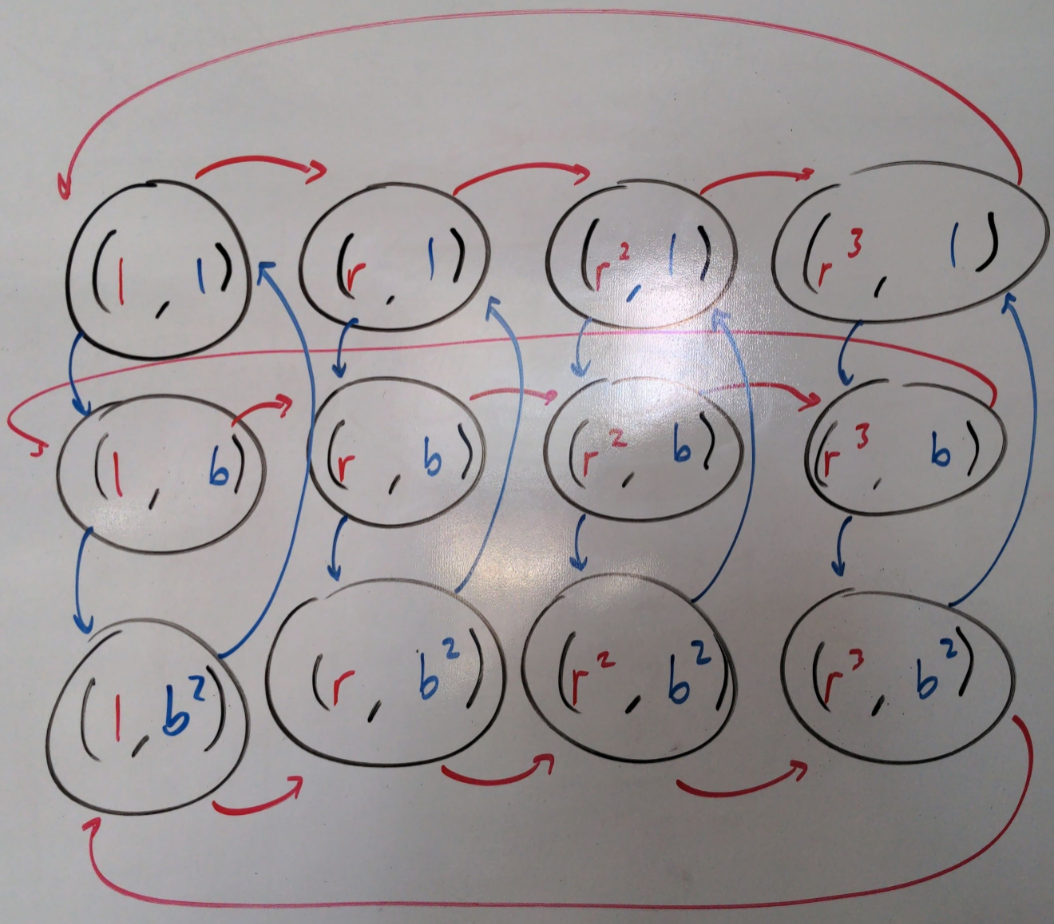
\includegraphics[width=0.5\textwidth]{../images/c4c3-ordered-pairs.png}
        \item (Bonus problem: Is $\Alert{C_4}\times \Balert{C_3}$ ``secretly cyclic''?) `'\begin{red}
            (Yes, it is generated by $(\Alert{r}, \Balert{b})$!)
        \end{red}
    \end{itemize}
\end{problem}

\begin{problem}
    Explore $\Alert{C_2} \times \Balert{C_2} \times \Galert{C_2}$.
    \begin{itemize}
        \item Figure out how to repeat the inflation process to draw a Cayley diagram.

        \begin{red}
            Can you tell that I was thinking of this as $(\Alert{C_2} \times \Balert{C_2}) \times \Galert{C_2}$? How do you think I would have drawn this a bit differently if I was thinking of it as $\Alert{C_2} \times (\Balert{C_2} \times \Galert{C_2})$?
        \end{red}

        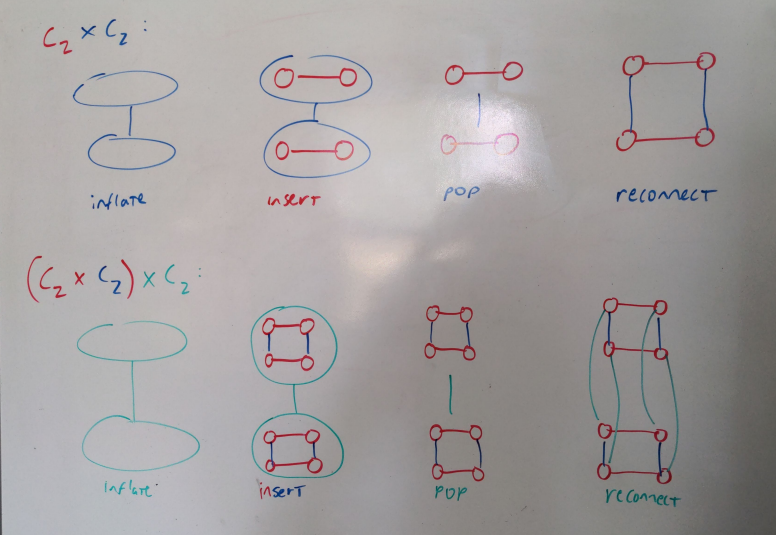
\includegraphics[width=0.7\textwidth]{../images/c2c2c2-inflation.png}
        \item Compute the orbits of each of the 8 elements and draw a cycle graph.

        I am thinking of $\Alert{C_2} = \<\Alert{r}\>$,  $\Balert{C_2} = \<\Balert{b}\>$, and $\Galert{C_2} = \<\Galert{g}\>$. 
        
        Challenge: think about $\Alert{\Z_2} \times \Balert{\Z_2} \times \Galert{\Z_2}$, written additively.

        \begin{minipage}{0.3\textwidth}
            \begin{tabular}{c|c}
                Element & Orbit \\
                $(\Alert{1}, \Balert{1}, \Galert{1}) = e$ & $\{e\}$ \\\hline
                $(\Alert{r}, \Balert{1}, \Galert{1})$ & $\{e, (\Alert{r}, \Balert{1}, \Galert{1})\}$ \\
                $(\Alert{1}, \Balert{b}, \Galert{1})$ & $\{e, (\Alert{1}, \Balert{b}, \Galert{1})\}$ \\
                $(\Alert{r}, \Balert{b}, \Galert{1})$ & $\{e, (\Alert{r}, \Balert{b}, \Galert{1})\}$ \\
                $(\Alert{1}, \Balert{1}, \Galert{g})$ & $\{e, (\Alert{1}, \Balert{1}, \Galert{g})\}$ \\
                $(\Alert{r}, \Balert{1}, \Galert{g})$ & $\{e, (\Alert{r}, \Balert{1}, \Galert{g})\}$ \\
                $(\Alert{1}, \Balert{b}, \Galert{g})$ & $\{e, (\Alert{1}, \Balert{b}, \Galert{g})\}$ \\
                $(\Alert{r}, \Balert{b}, \Galert{g})$ & $\{e, (\Alert{r}, \Balert{b}, \Galert{g})\}$ \\
            \end{tabular}
        \end{minipage}
        \begin{minipage}{0.7\textwidth}
            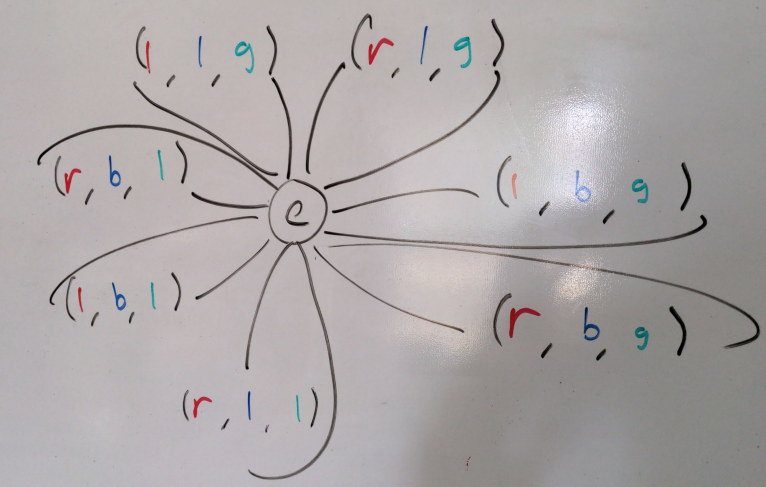
\includegraphics[width=\textwidth]{../images/c2c2c2-cycle.png}
        \end{minipage}
        \item Is this a new group? Groups of order 8 we already know are $C_8$, $C_4 \times C_2$, $D_4$, and $Q_8$. 

        \begin{red}
            This is definitely a new group, because everybody in this group has order 2 (as is easy to see in the cycle graph), but that's not true of any of the other groups of order 8 we know!
        \end{red}
    \end{itemize}
\end{problem}

\begin{problem}
    Prove using algebra that $A\times B$ is abelian \Alert{if and only if} both $A$ and $B$ are abelian.

    \textit{Hint:} Remember that an \Alert{``if and only if''} statement is actually looking for \textit{two} proofs.

    \begin{red}
        Same note as previously: Please note that I am writing out the details of this proof very carefully, so that it is clear at each step what is my data and what is my claim. As is usual, most of the warrants are ``implicit;'' see if you can fill in the warrants that connect the data to the claims.
    \end{red}
    \begin{multicols}{2}
        ($\Rightarrow$) Suppose that $A$ and $B$ are both abelian.

        \begin{red}
            Let $a, x\in A$ and $b, y\in B$. 
            
            Since $A$ and $B$ are abelian,
            \[ax = xa \text{ and } by = yb.\]

            Consider $(a, b), (x, y)\in A\times B$.
            \begin{align*}
                (a, b)\cdot(x, y) &= (ax, by) \\
                &= (xa, yb) \\
                &= (x, y) \cdot (a,b).
            \end{align*}
        \end{red}
        Therefore, $A\times B$ is abelian.

        \columnbreak

        ($\Leftarrow$) Suppose that $A\times B$ is abelian.

        \begin{red}
            Let $(a, b), (x, y)\in A\times B$. 
            
            Since $A\times B$ is abelian, \[(a, b)\cdot(x, y) = (x, y) \cdot (a,b).\]
                
            But then $(ax, by) = (xa, yb)$,

            so $ax = xa$, 

            and $by = yb$.
        \end{red}

        Therefore, $A$ and $B$ are both abelian.
    \end{multicols}
    
\end{problem}

\begin{problem}
    Here we'll explore when the product of cyclic groups is ``secretly cyclic''.

    \begin{red}
        Same note as previously: Please note that I am writing out the details of this proof very carefully, so that it is clear at each step what is my data and what is my claim. As is usual, most of the warrants are ``implicit;'' see if you can fill in the warrants that connect the data to the claims.
    \end{red}
    \begin{enumerate}[(a)]
        \item Say you have a generic group $G$ such that $|G| = n$. Suppose further that you found an element $g\in G$ such that $|g| = n$. Prove that $G$ is cyclic. (Hint: look at the orbit of $g$, and think about the definition of $|g|$.)

        \begin{red}
            Since $|g| = n$, we know $g^n = e$ and $g^k \neq e$ for any $k < n$. Therefore, the orbit of $g$ is $\<g\> = \{g, g^2, \ldots, g^{n-1}, g^n = e \}$, and all those powers of $g$ are distinct.

            (How do we know all those powers are distinct? If $g^a = g^b$ for some $a, b < n$, then $g^{b-a} = e$ with $b-a<n$, but that contradicts the fact that $|g| = n$.)

            $g^k \in G$ for every $k\in \Z$, so this list of $n$ distinct elements must be precisely all of $G$. 

            Therefore, $G = \<g\>$, so $G$ is cyclic.
        \end{red}

        \item Suppose that $a, b \in \Z$ are relatively prime. (Google it if you don't remember what this means.) Fact: $\lcm(a, b) = ab.$ Optional challenge: prove it.

        \begin{red}
            This proof is actually somewhat involved! You have to know the ``Euclidean algorithm'' aka integer division with remainder. That's why it was optional. :)
        \end{red}

        \item Consider the direct product $\Z_a \times \Z_b$, with $a$ and $b$ relatively prime. What is $|(1,1)|$?

        (\textbf{\Alert{NOTE TYPO FIX:}} I had previously written $C_a \times C_b$, in which the element $(1,1)$ would represent the identity. I could also have said, suppose that $C_a = \<g\>$ and $C_b = \<h\>$ and then think about the element $(g, h)\in C_a \times C_b$, but I think it's cleaner this way.)

        \begin{red}
            Okay so here's the deal. The main reason I wanted to write this key was to resolve the issue with the typo here. I am going to write this proof two ways: first with the groups \textbf{written additively}, as suggested here, and then \Balert{\textbf{written multiplicatively}.}

            \textbf{Written additively}: $\Z_a$ and $\Z_b$ are both generated by repeatedly adding the element $1$, but in $\Z_a$, $|1| = a$, and in $\Z_b$, $|1| = b$. To help us distinguish between these two different versions of $1$, I'm going to write $\Z_a = \<1_a\>$ and $\Z_b = \<1_b\>$; note in particular that $1_a \cdot a = 0$ and $1_b \cdot b = 0$ (because 0 is the identity element here).

            Consider the element $(1_a, 1_b) \in \Z_a \times \Z_b$. I claim that $|(1_a, 1_b)| = \lcm(a, b)$. By the definition of order, $|(1_a, 1_b)|$ is the smallest $k$ such that $(1_a\cdot k, 1_b \cdot k) = (0, 0)$. But looking in the $\Z_a$ component, this means that $k$ is a multiple of $a$, and looking in the $\Z_b$ component, this means that $k$ is a multiple of $b$. Therefore, $k$ is a common multiple of $a$ and $b$, and since $k$ is the \textit{least} such number, $k = \lcm(a, b)$.

            Since $a$ and $b$ are relatively prime, $\lcm(a, b) = ab$, so $k = ab$, so $|(1_a, 1_b)| = ab$.
        \end{red}

        \begin{xBlue}
            \textbf{Written multiplicatively}: Very similar. I literally am copy-pasting and modifying.

            $C_a = \<g\>$ and $C_b = \<h\>$ are both generated by repeatedly multiplying their generating element. In $C_a$, $|g| = a$, and in $C_b$, $|h| = b$. Note in particular that $g^a = e$ and $h^b = e$ because $e$ is the name of the identity element here.

            Consider the element $(g, h) \in C_a \times C_b$. I claim that $|(g, h)| = \lcm(a, b)$. By the definition of order, $|(g,h)|$ is the smallest $k$ such that $(g^k, h^k) = (e, e)$. But looking in the $C_a$ component, this means that $k$ is a multiple of $a$, and looking in the $C_b$ component, this means that $k$ is a multiple of $b$. Therefore, $k$ is a common multiple of $a$ and $b$, and since $k$ is the \textit{least} such number, $k = \lcm(a, b)$.

            Since $a$ and $b$ are relatively prime, $\lcm(a, b) = ab$, so $k = ab$, so $|(g, h)| = ab$.
        \end{xBlue}

        \item Conclude that $\Z_a \times \Z_b \cong \Z_{ab}.$

        \begin{red}
            Finally, we can apply the result of part (a) to conclude that since $|\Z_a \times \Z_b| = ab$, and since $|(1_a, 1_b)| = ab$, $\Z_a \times \Z_b$ is cyclic, generated by $(1_a, 1_b)$. Therefore, $\Z_a \times \Z_b \cong \Z_{ab}$, the (additive) cyclic group of order $ab$.
        \end{red}

        \begin{xBlue}
            Finally, we can apply the result of part (a) to conclude that since $|C_a \times C_b| = ab$, and since $|(g, h)| = ab$, $C_a \times C_b$ is cyclic, generated by $(g, h)$. Therefore, $C_a \times C_b \cong C_{ab}$, the (multiplicative) cyclic group of order $ab$.
        \end{xBlue}
    \end{enumerate}
\end{problem}

\end{document}

